% Class file
\documentclass[11pt,a4paper]{jsarticle}
% -----------------------------------------------------------------------

\def\rlsTex{../../rlsTex}
\input{\rlsTex/setup/meeting}

\graphicspath{{../../fig/}{./fig/}}

\renewcommand{\meetingtitle}{Meeting}
\renewcommand{\meetingauthor}{Hirai Haruki}
% -----------------------------------------------------------------------
%
%%%%%%%%%%%%%%%%%%%%%%%%%%%%%%%%%%%%%%%%%%%%%%%%%%%%%%%%%%%%%%%%%%%%%%%%
\begin{document}
\header

\section{諸言}
人型ロボットの歩行制御において様々な研究がなされいる.また,本研究室でもDCMおよびVRPを指標としたシミュレーション環境での歩行制御が実現されている.
実環境での確認のため実機での実験が求められるが,転倒によるギアの故障や許容トルクを超えることによるモータの破損を回避しなければならない.
よって,許容トルクの確認など慎重な準備が必要である.
本研究では,実環境での適応において人型ロボットの基本動作である二足歩行を,実験機において実現させることを目的とする.
本稿では,歩行動作時の関節における干渉についての確認を行う.その後,非干渉となるパラメータを明確にする.

\section{干渉確認}
干渉確認モデルを用いた歩行動作を行った際の干渉時を以下に示す.また,今回シミュレーション条件をTable~\ref{tab:table1}に示した.
\begin{table}[h]
  \centering
  \caption{Simulated conditions in walking motion.}
  \vspace{-2mm}
  \begin{tabular}[t]{|c|c|c|c|c|c|}
    \hline
    $T_{step}$ [s]& $T_{DS}$ [s]& $T_{SS}$ [s]& Stride [m] & VRPoffset [m]\\ \hline
    0.5 & 0.2 & 0.3 & 0.08 & 0.022\\ \hline
  \end{tabular}
  \label{tab:table1}
\end{table}

\newpage
\begin{figure}[h]
  \begin{minipage}{0.45\linewidth}
    \centering
    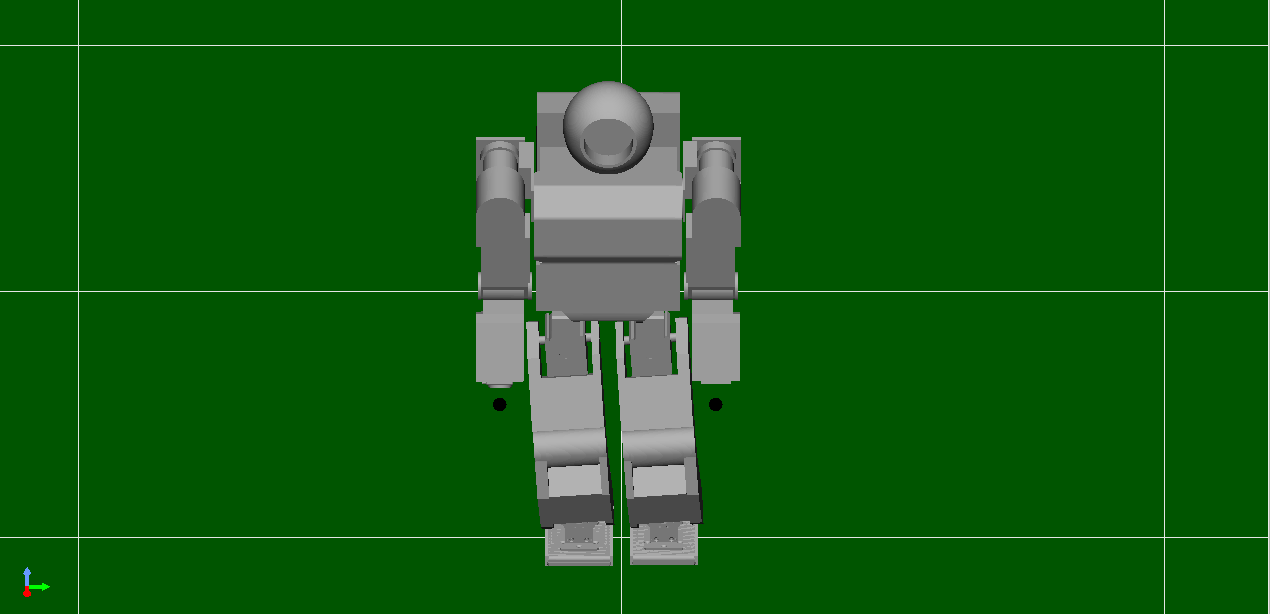
\includegraphics[width=1.0\linewidth]{./fig/coupled.png}
    \footnotesize{\hspace{30pt}(a)}
  \end{minipage}
  \begin{minipage}{0.1\linewidth}
    \centering
    \hspace{-0.1mm}
  \end{minipage}
  \begin{minipage}{0.45\linewidth}
    \centering
    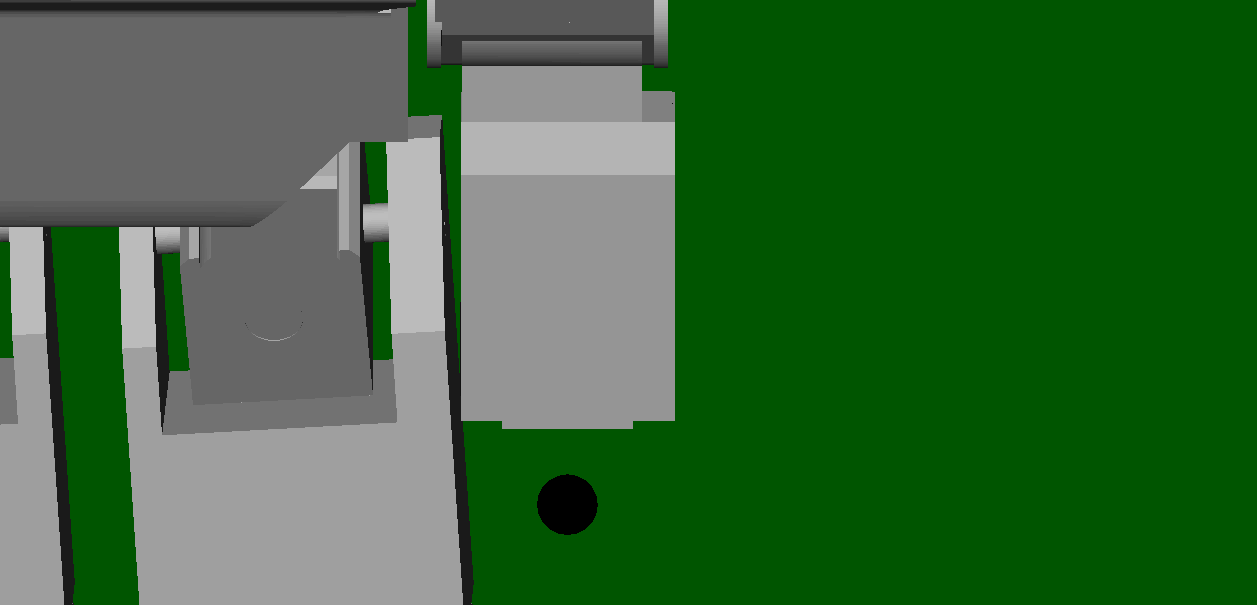
\includegraphics[width=1.0\linewidth]{./fig/01V2.png}
    \footnotesize{\hspace{30pt}(b)}
  \end{minipage}
  \caption{Model view of coupled walking.}
  \label{fig:No1}
\end{figure}


\begin{figure}[h]
  \begin{minipage}{0.45\linewidth}
    \centering
    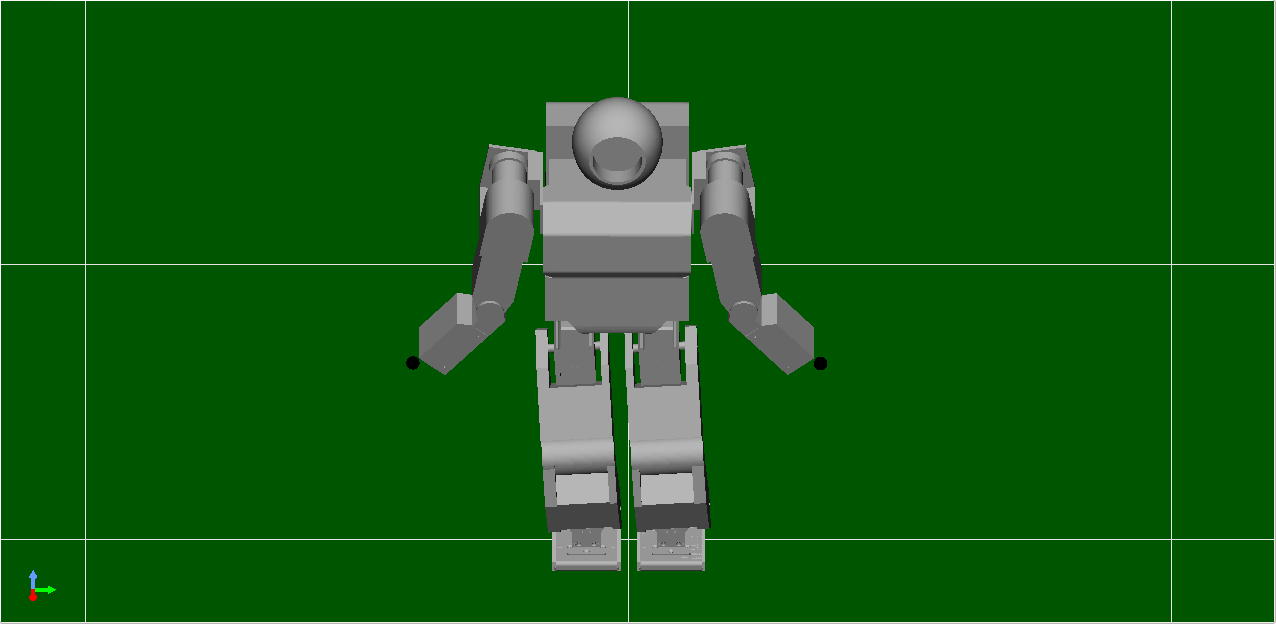
\includegraphics[width=1.0\linewidth]{./fig/decoupled.png}
    \footnotesize{\hspace{30pt}(a)}
  \end{minipage}
  \begin{minipage}{0.1\linewidth}
    \centering
    \hspace{-0.1mm}
  \end{minipage}
  \begin{minipage}{0.45\linewidth}
    \centering
    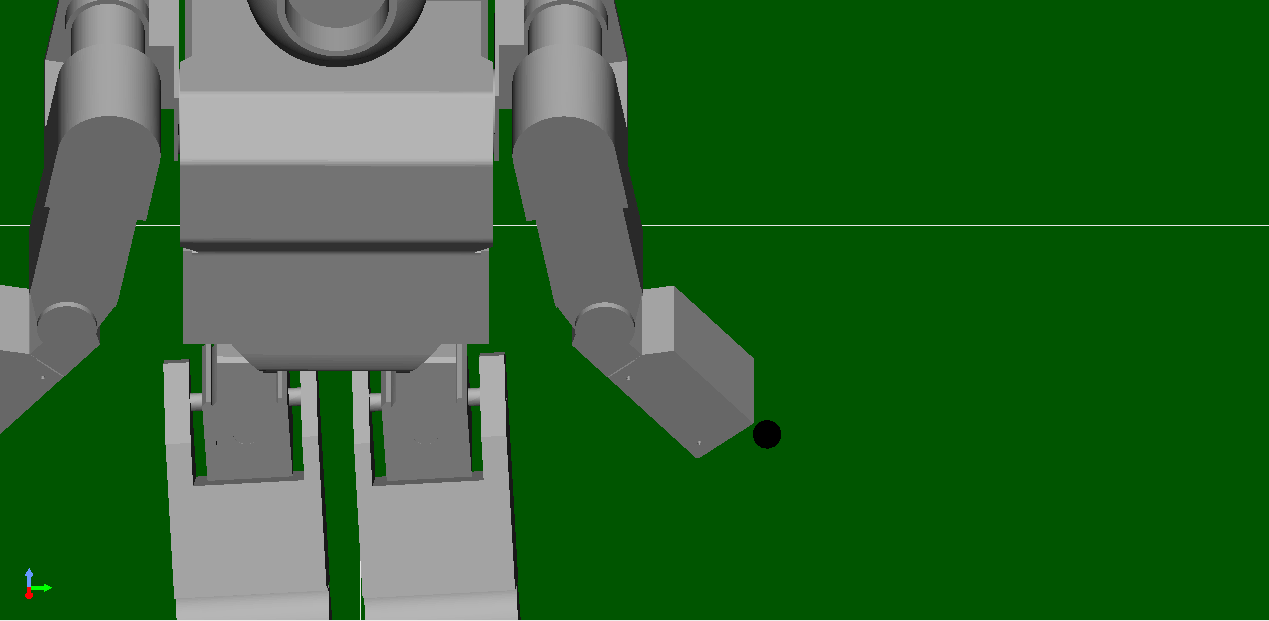
\includegraphics[width=1.0\linewidth]{./fig/decoupled2.png}
    \footnotesize{\hspace{30pt}(b)}
  \end{minipage}
  \caption{Model view of decoupled walking.}
  \label{fig:No1}
\end{figure}

\noindent
以上より左腕関節と左脚関節が干渉していることがわかる.
% ####################################################
% テンプレート
% \cite{kajita2003}
% \section{図}
% \label{subsec:figure}
% % ##############################################
% 図を単体で挿入する場合,
% 複数の図を一つのFigとして示す場合,
% ファイルの枠組みを無視して図を挿入する場合をそれぞれ
% Fig.~\ref{fig:model},
% Fig.~\ref{fig:minipage},
% Fig.~\ref{fig:forcedInsert}に示す.
% \begin{figure}[h]
%   % 図を挿入場所は b:bottom, h:hear, t:top, p:pageを用いて調整
%   \centering
%   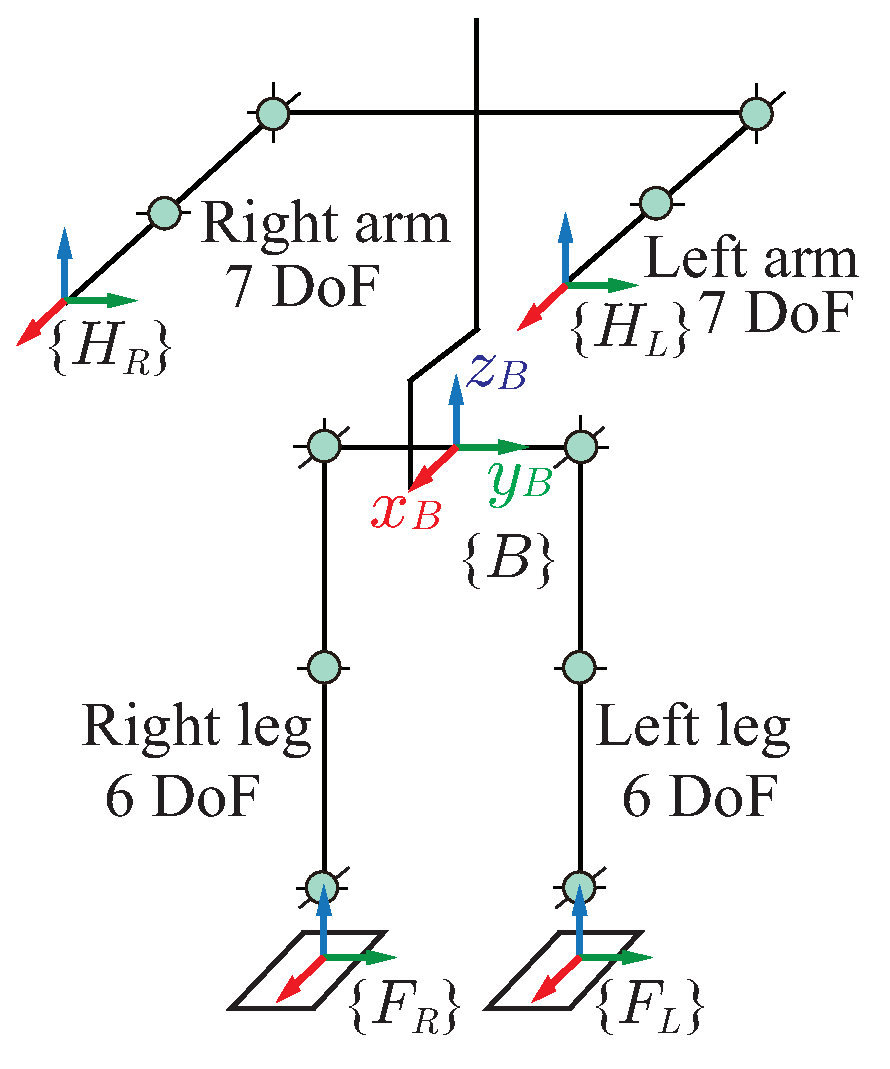
\includegraphics[width=0.5\linewidth]{./fig/hoap2model.eps}
%   % 画像ファイルの相対パス
%   \caption{Sample figure.}
%   % 画像のキャプション
%   \label{fig:model}
%   % 文中で参照する場合に用いる
% \end{figure}
% % ..............................................
% % ==============================================
% \begin{figure}[t]
% \centering
% \begin{minipage}{0.2\linewidth}
%     \centering
%     \includegraphics[width=0.95\linewidth]{./key/workKey.eps}
%   \end{minipage}\\
% %
%   \begin{minipage}{0.45\linewidth}
%     \centering
%     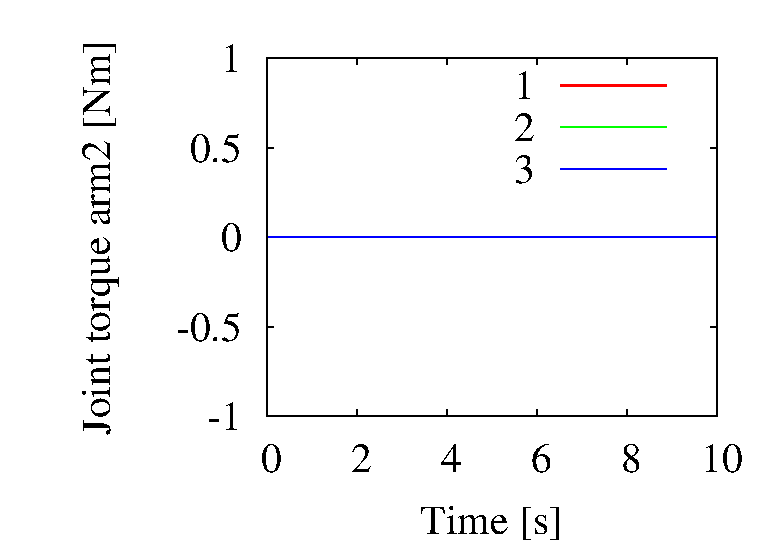
\includegraphics[width=0.95\linewidth]{./fig/result1.eps}
%     \footnotesize{\hspace{30pt}(a)}
%   \end{minipage}
%   \begin{minipage}{0.45\linewidth}
%     \centering
%     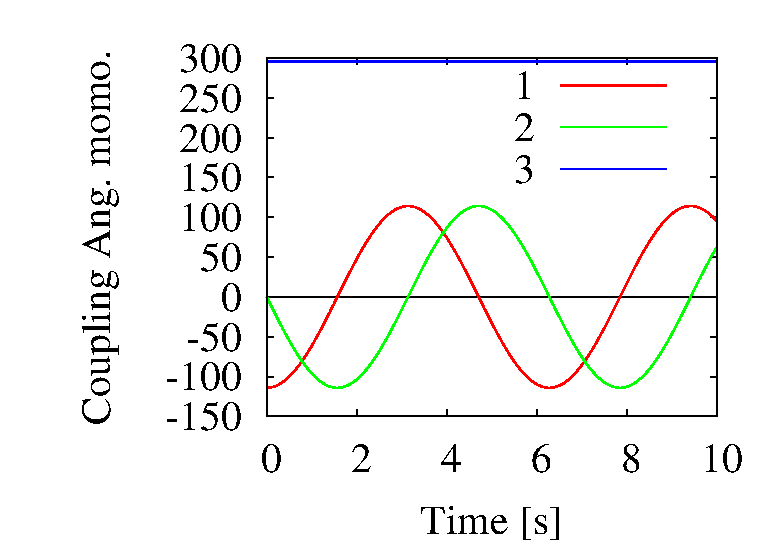
\includegraphics[width=0.95\linewidth]{./fig/result2.eps}
%     \footnotesize{\hspace{30pt}(b)}
%   \end{minipage}
%   \caption{Simulation results: (a) joint torque and (b) angular momentum.}
%   \label{fig:minipage}
% \end{figure}
% % ..............................................
% % ==============================================
% \begin{figure*}[t]
%   \begin{minipage}{0.333\linewidth}
%     \centering
%     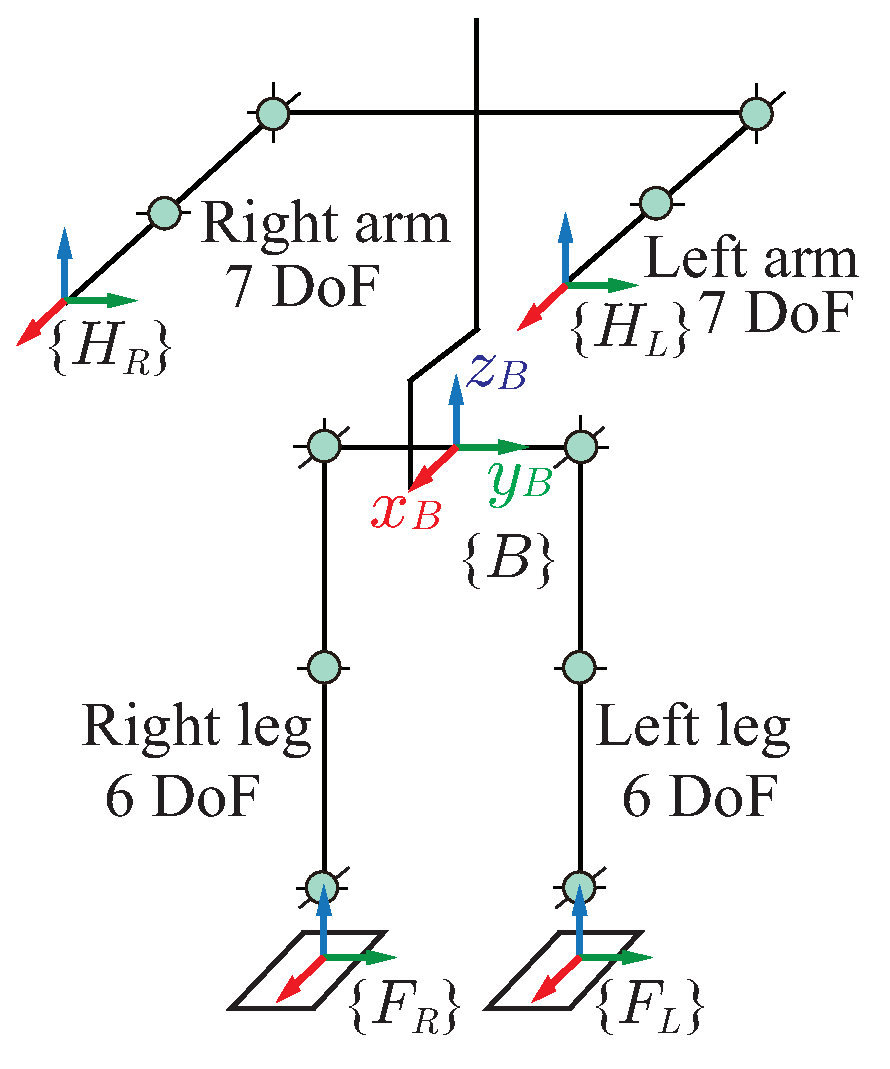
\includegraphics[width=1.0\linewidth]{./fig/hoap2model.eps}
%     \footnotesize{(a)}
%   \end{minipage}
%   \begin{minipage}{0.333\linewidth}
%     \centering
%     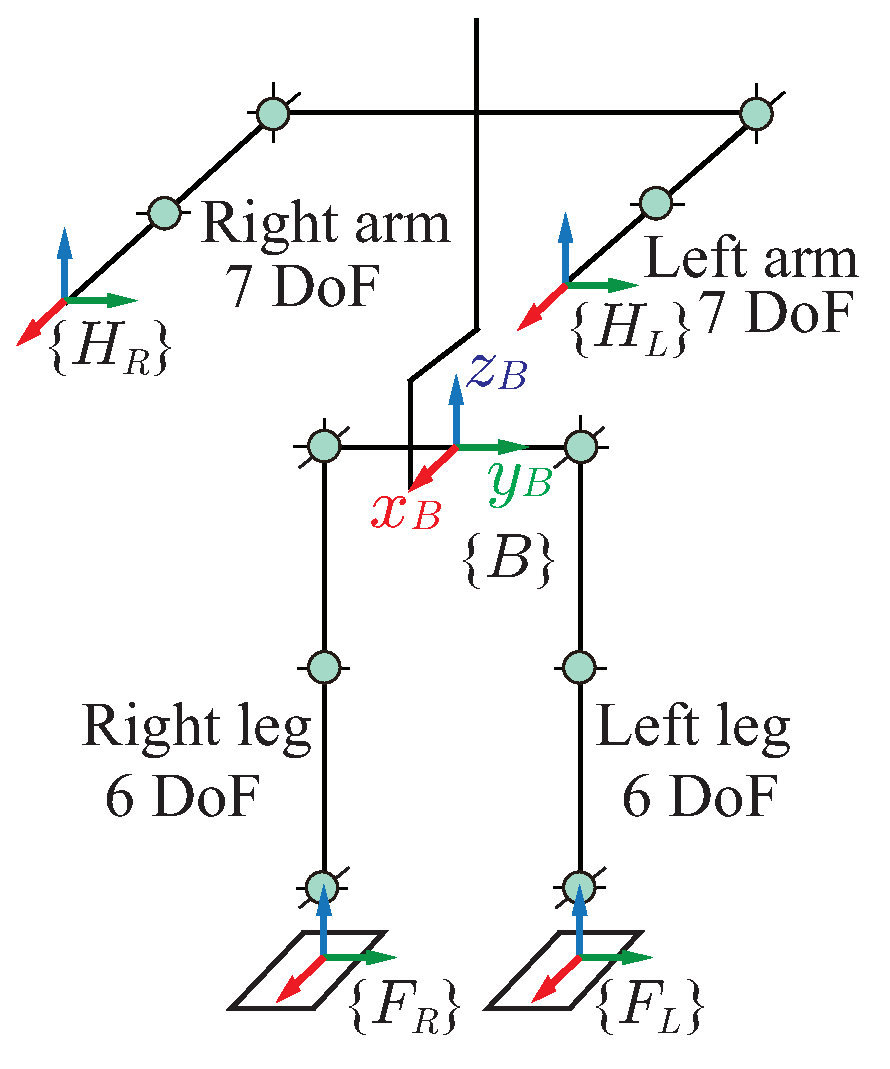
\includegraphics[width=1.0\linewidth]{./fig/hoap2model.eps}
%     \footnotesize{(b)}
%   \end{minipage}
%   \begin{minipage}{0.333\linewidth}
%     \centering
%     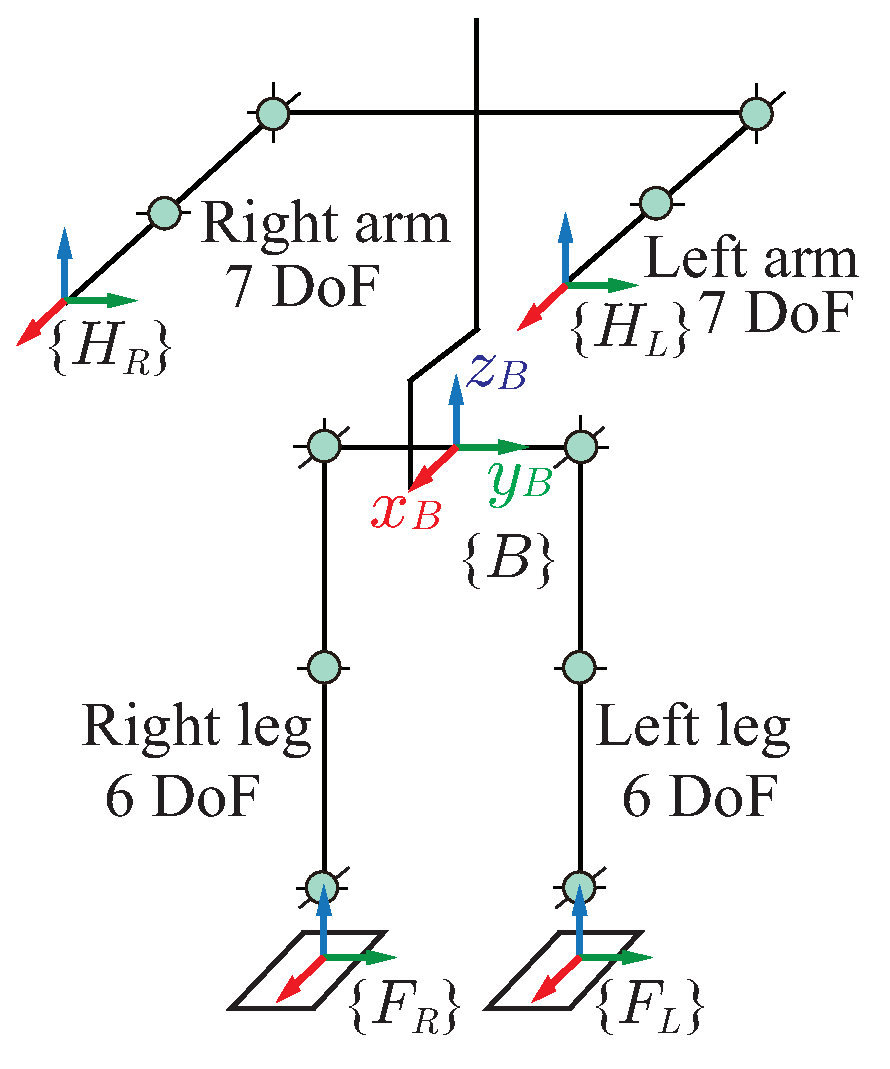
\includegraphics[width=1.0\linewidth]{./fig/hoap2model.eps}
%     \footnotesize{(c)}
%   \end{minipage}
%   \caption{Sample figure 3: (a) HOAP-2 1, (b) HOAP-2 2 and (c) HOAP-2 3.}
%   \label{fig:forcedInsert}
% \end{figure*}
% % ..............................................

% \clearpage
% \section{rlsTex内に定義されたマクロの使用例}
% texs直下にあるrlsTex/mydef内で定義されているマクロの使用例です.
% texの使い方に慣れてきたらマクロを自分で設定して使ってみてください.
% \subsection{浮遊ベースロボットの運動方程式}
% \bal[eom]{
%   \bmMM[exp2]\ddbmqM[exp2] + \bmcM[exp2] + \bmgC[exp2] = \bmQ[exp2] + \bmJcM[exp2][T]\obmcalFc
% }

% \eqRef{eom}
% \subsection{図}
% \bfig{h}{
%   \ig{0.3}{model/skeletonA7.eps}
% }{
%   Caption
% }

% \bfig{h}[result]{
%   \bmpnsc{t}{1.}{
%     \ig{.2}{key/workKey.eps}
%   }
%   \bmpsc{t}{1.}{
%     \ig{.3}{model/skeletonA7.eps}
%   }
% }{
%   Caption
% }

% \figRef{result}

% \href{run:movie/test.mp4}{Link}

% %%%%%%%%%%%%%%%%%%%%%%%%%%%%%%%%%%%%%%%%%%%%%%%%%%%%%%%%%%%%%%%%%%%%%%%%
% % ======================================================
% % .................How to Hyper link....................
% % \href{URL}{\cite{name}}

% % ======================================================
% \newpage
% %% reference
% \bibliographystyle{junsrt}
% \input{\rlsbib/wrapper/humanoid}
% %
% %%%%%%%%%%%%%%%%%%%%%%%%%%%%%%%%%%%%%%%%%%%%%%%%%%%%%%%%%%%%%%%%%%%%%%%%
% %
\end{document}
% %
% %
%
Local Variables:
mode: japanese-latex
TeX-master: t
End:
